\subsection{Wave-breaking field}
\underline{Dawson's derivation} [Note: The wave-breaking field does not represent the onset of the non-linear regime but the highest achievable field in the non-linear regime.]
We consider a simple 1D linear non-relativistic electron sheet model first used by Dawson \citep{Dawson1959} to show the breakdown of the linear model (\textcolor{red}{correct?}). Consider the plasma being made up of thin sheets of ions and electrons. A sheet at equilibrium position $z=z_0$ is then displaced by $\eta_0(z_0)$, where the displacement is set as function of the equilibrium position for full generality, to a new position $z=z_0+\eta_0$. The displaced sheet reveals a positive surface charge density $\sigma=en_0\eta_0$, where $n_0$ is the electron charge density in the plasma. This sets up a restoring electric field which we find using Gauss's law to be $E_{\text{res}}=4\pi n_0e\eta_0$ which yields a restoring force
\begin{equation}
 m_e\frac{\partial^2\eta_0}{\partial t^2}=-eE_{\text{res}}=-4\pi n_0e^2\eta_0=-\omega_p^2\eta_0
 \end{equation} 
 with solutions 
 \begin{equation}
 \eta_0(z_0,t)=A_1(z_0)\cos(\omega_p t)+A_2(z_0)\sin(\omega_p t)
 \end{equation}
The phenomena of wave breaking can be shown by considering another electron sheet at an equilibrium position $z_1=z_0+\Delta z_0$ at a distance $\Delta z_0$ away from the first sheet. This sheet is then displaced by $\eta_1$ to a new position $z^{*}_1=z_0+\Delta z_0+\eta_1$. The linear model is valid provided that there are no electron trajectories intersect one another in the plasma [ \textcolor{red}{is this correct? Why does the model break down?} ]. Hence the model is valid provided that $z^{*}_1-z_0>z-z_0$ which implies that we must have
\begin{equation}
\Delta z_0+\eta_1>\eta_0~,
\label{eta_ineq}
\end{equation}
for all $\Delta z_0\in \mathbb{R}$, to sustain plasma oscillations in the linear model. We now consider  the limit as $\Delta z_0\to 0$ for the expression 
\begin{equation}
\frac{\partial \eta}{\partial x_0}=\lim_{\Delta z_0\to 0}\frac{\Delta \eta}{\Delta z_0}=\lim_{\Delta z_0\to 0}\left(\frac{\eta_1-\eta_0}{\Delta z_0}\right)>\lim_{\Delta z_0\to 0}\left(\frac{\eta_0-\Delta z_0-\eta_0}{\Delta z_0}\right)=-1
\end{equation}
which simplifies to
\begin{equation}
\frac{\partial \eta}{\partial z_0}>-1
\label{no_crossing}
\end{equation}
where the inequality is introduced using Eq. (\ref{eta_ineq}). We now consider the special case where $A_1(z_0)=A\sin(k_pz_0)$ and $A_2(z_0)=0$. This is a valid solution since $\sin(k_pz_0)$ is single-valued for all $k_p,x_0\in\mathbb{R}$. This particular solution is chosen to highlight the breadown of the electric field, and is motivated by ([\textcolor{red}{what?}]) the solution we found for the electric field in section 2. Applying the no-crossing criterion in Eq. \ref{no_crossing} to $\eta=\eta_0(z_0,t)$ yields
\begin{equation}
\frac{\partial \eta_0}{\partial z_0}=Ak_p\cos(k_pz_0)>-1 \quad \Leftrightarrow \quad Ak_p\leq 1
\end{equation}
which gives the maximum amplitude as $A_{max}=1/k_p$. Hence the maximum restoring electric field $E_{max}\equiv E_{\text{wb}}=4\pi n_0/k_p$ is given by
\begin{equation}
E_{\text{wb}}=\frac{m_ev_p\omega_p}{e}
\end{equation}
the so-called \textit{wave-breaking field}. To further show how this breaks the linear model we consider the effect on the electric field up to and past the wave-breaking limit. As above we have, 
\begin{equation}
z=z_0+\eta_0=z_0+A\sin(k_p z_0)
\label{dawson_z}
\end{equation}
and 
\begin{equation}
E=4\pi n_0e A\sin(k_p z_0)
\label{dawson_E(z)}
\end{equation}
from which we want to find the electric field as a function of $z$. We can do this by numerically solving Eq. \ref{dawson_z} for $z_0$ in a range of $z$ values given fixed values of $A$. The gives $z_0=z_0(z,A)$ which can be substituted into Eq. \ref{dawson_E(z)} to give $E=E(z,A)$, the result of which is shown in Fig. \ref{DawsonCriterionPlot}. From this we conclude that the electric field is no longer single-valued for $A>1/k_p$, i.e past the electric field's wave-breaking amplitude, which signifies a breakdown of the linear model.\\
This is further emphasized by consider the electron-density response as $\partial \eta/\partial z_0\to -1$. To do this we use  Eq. XXX in 1D with no beam density $n_b=0$, 
\begin{equation}
\frac{\partial E}{\partial z}=4\pi e(n_0-n)
\end{equation}
where $n=n_0+n_1$ is the perturbed plasma density and $n_0$ is the ion density, hence $n_0-n$ is the free (negative) charge density in the plasma. We now take the derivative of the perturbed electric field and substitute the above expression
\begin{equation}
\frac{\partial E}{\partial z}=4\pi n_0 e \frac{\partial \eta}{\partial z} \quad \Rightarrow \quad n=n_0\left(1-\frac{\partial \eta}{\partial z}\right)
\end{equation}
We now rewrite $\partial /\partial z$, using $z=z_0+\eta$, as
\begin{equation}
\frac{\partial}{\partial z}=\left(1-\frac{\partial \eta }{\partial z_0}\right)^{-1}\frac{\partial}{\partial z_0}
\end{equation}
which gives
\begin{equation}
n=\frac{n_0}{1+\frac{\partial \eta }{\partial z_0}}
 \end{equation} 
 which means that the perturbed electron density grows infinite as $\partial \eta/\partial z_0\to -1$, again signifying the breakdown of the linear model.\\
\\
Having seen that the linear theory can break down mathematically, it is crucial to ask whether this is realised in 3D models and experiments as well. 
\begin{figure}
\centering
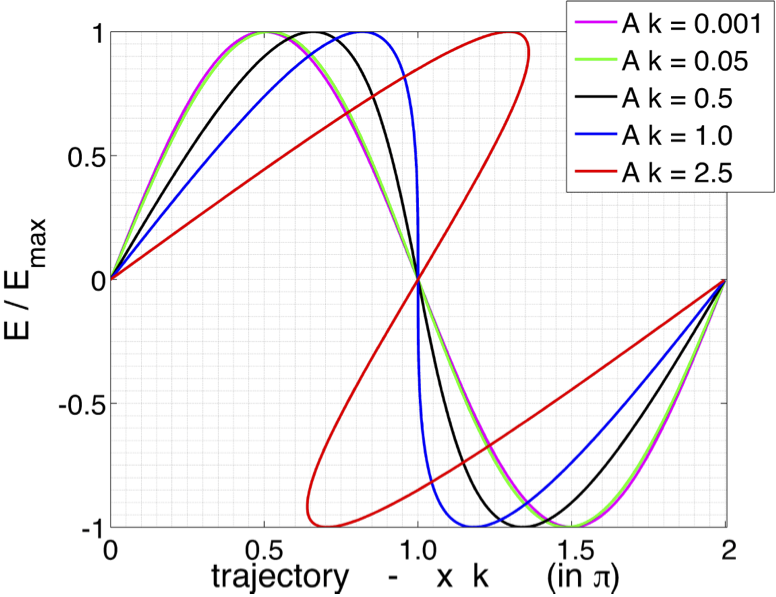
\includegraphics[scale=1]{SahaiThesisPlot.png}
\caption{Plot corresponding to Dawson's derivation of the wave-breaking field [ref. Sahai].}
\label{DawsonCriterionPlot}
\end{figure}

\clearpage
\section{Particle interactions with matter}
Conventional beam dumps work by stochastic interactions of the beam with the dense medium [hanahoe 6.5]
\subsection{Bohr-Fermi-Bethe-Bloch Theory}
Bethe-Bloch forumla:
\begin{equation}
-\expval{\frac{\mathrm{d}U}{\mathrm{d}s}}_{\text{ion}}=\frac{4\pi e^4n_{e,m}}{m_ec^2\beta^2}\left[\ln\left(\frac{2m_e\gamma^2v^2}{I}\right) -\beta^2\right]
\end{equation}

\subsection{Collective Plasma Deceleration -- Non-Linear regime }
\clearpage
\begin{figure}
\centering
\includegraphics[width=1.15\textwidth]{visit0098.pdf}
\caption{Non-linear regime, plasma density perturbations. Added custom legend with density=number of electrons / grid-square size. }
\end{figure}

\begin{figure}
\centering
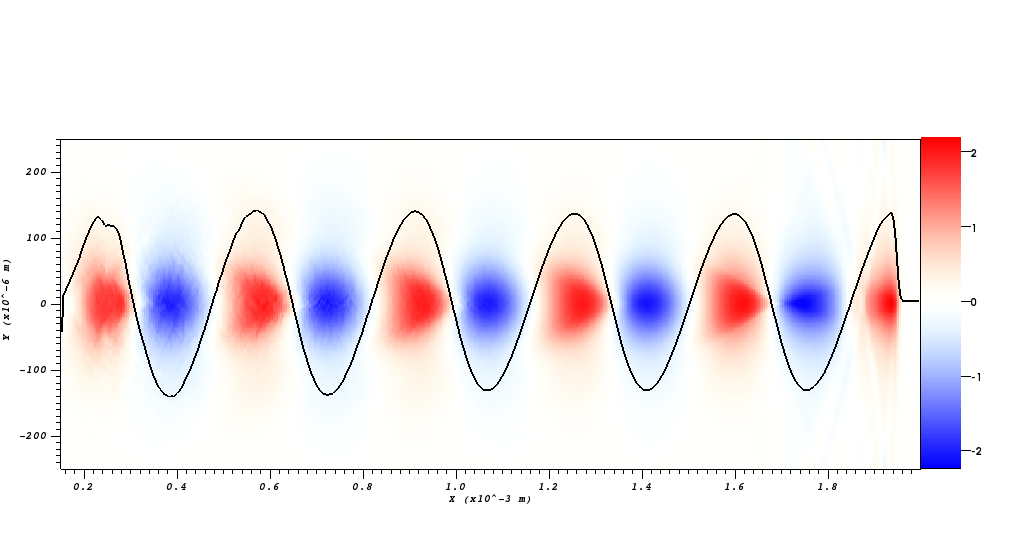
\includegraphics[width=\textwidth]{Ex_nonlinear.png}
\end{figure}
\begin{figure}
\centering
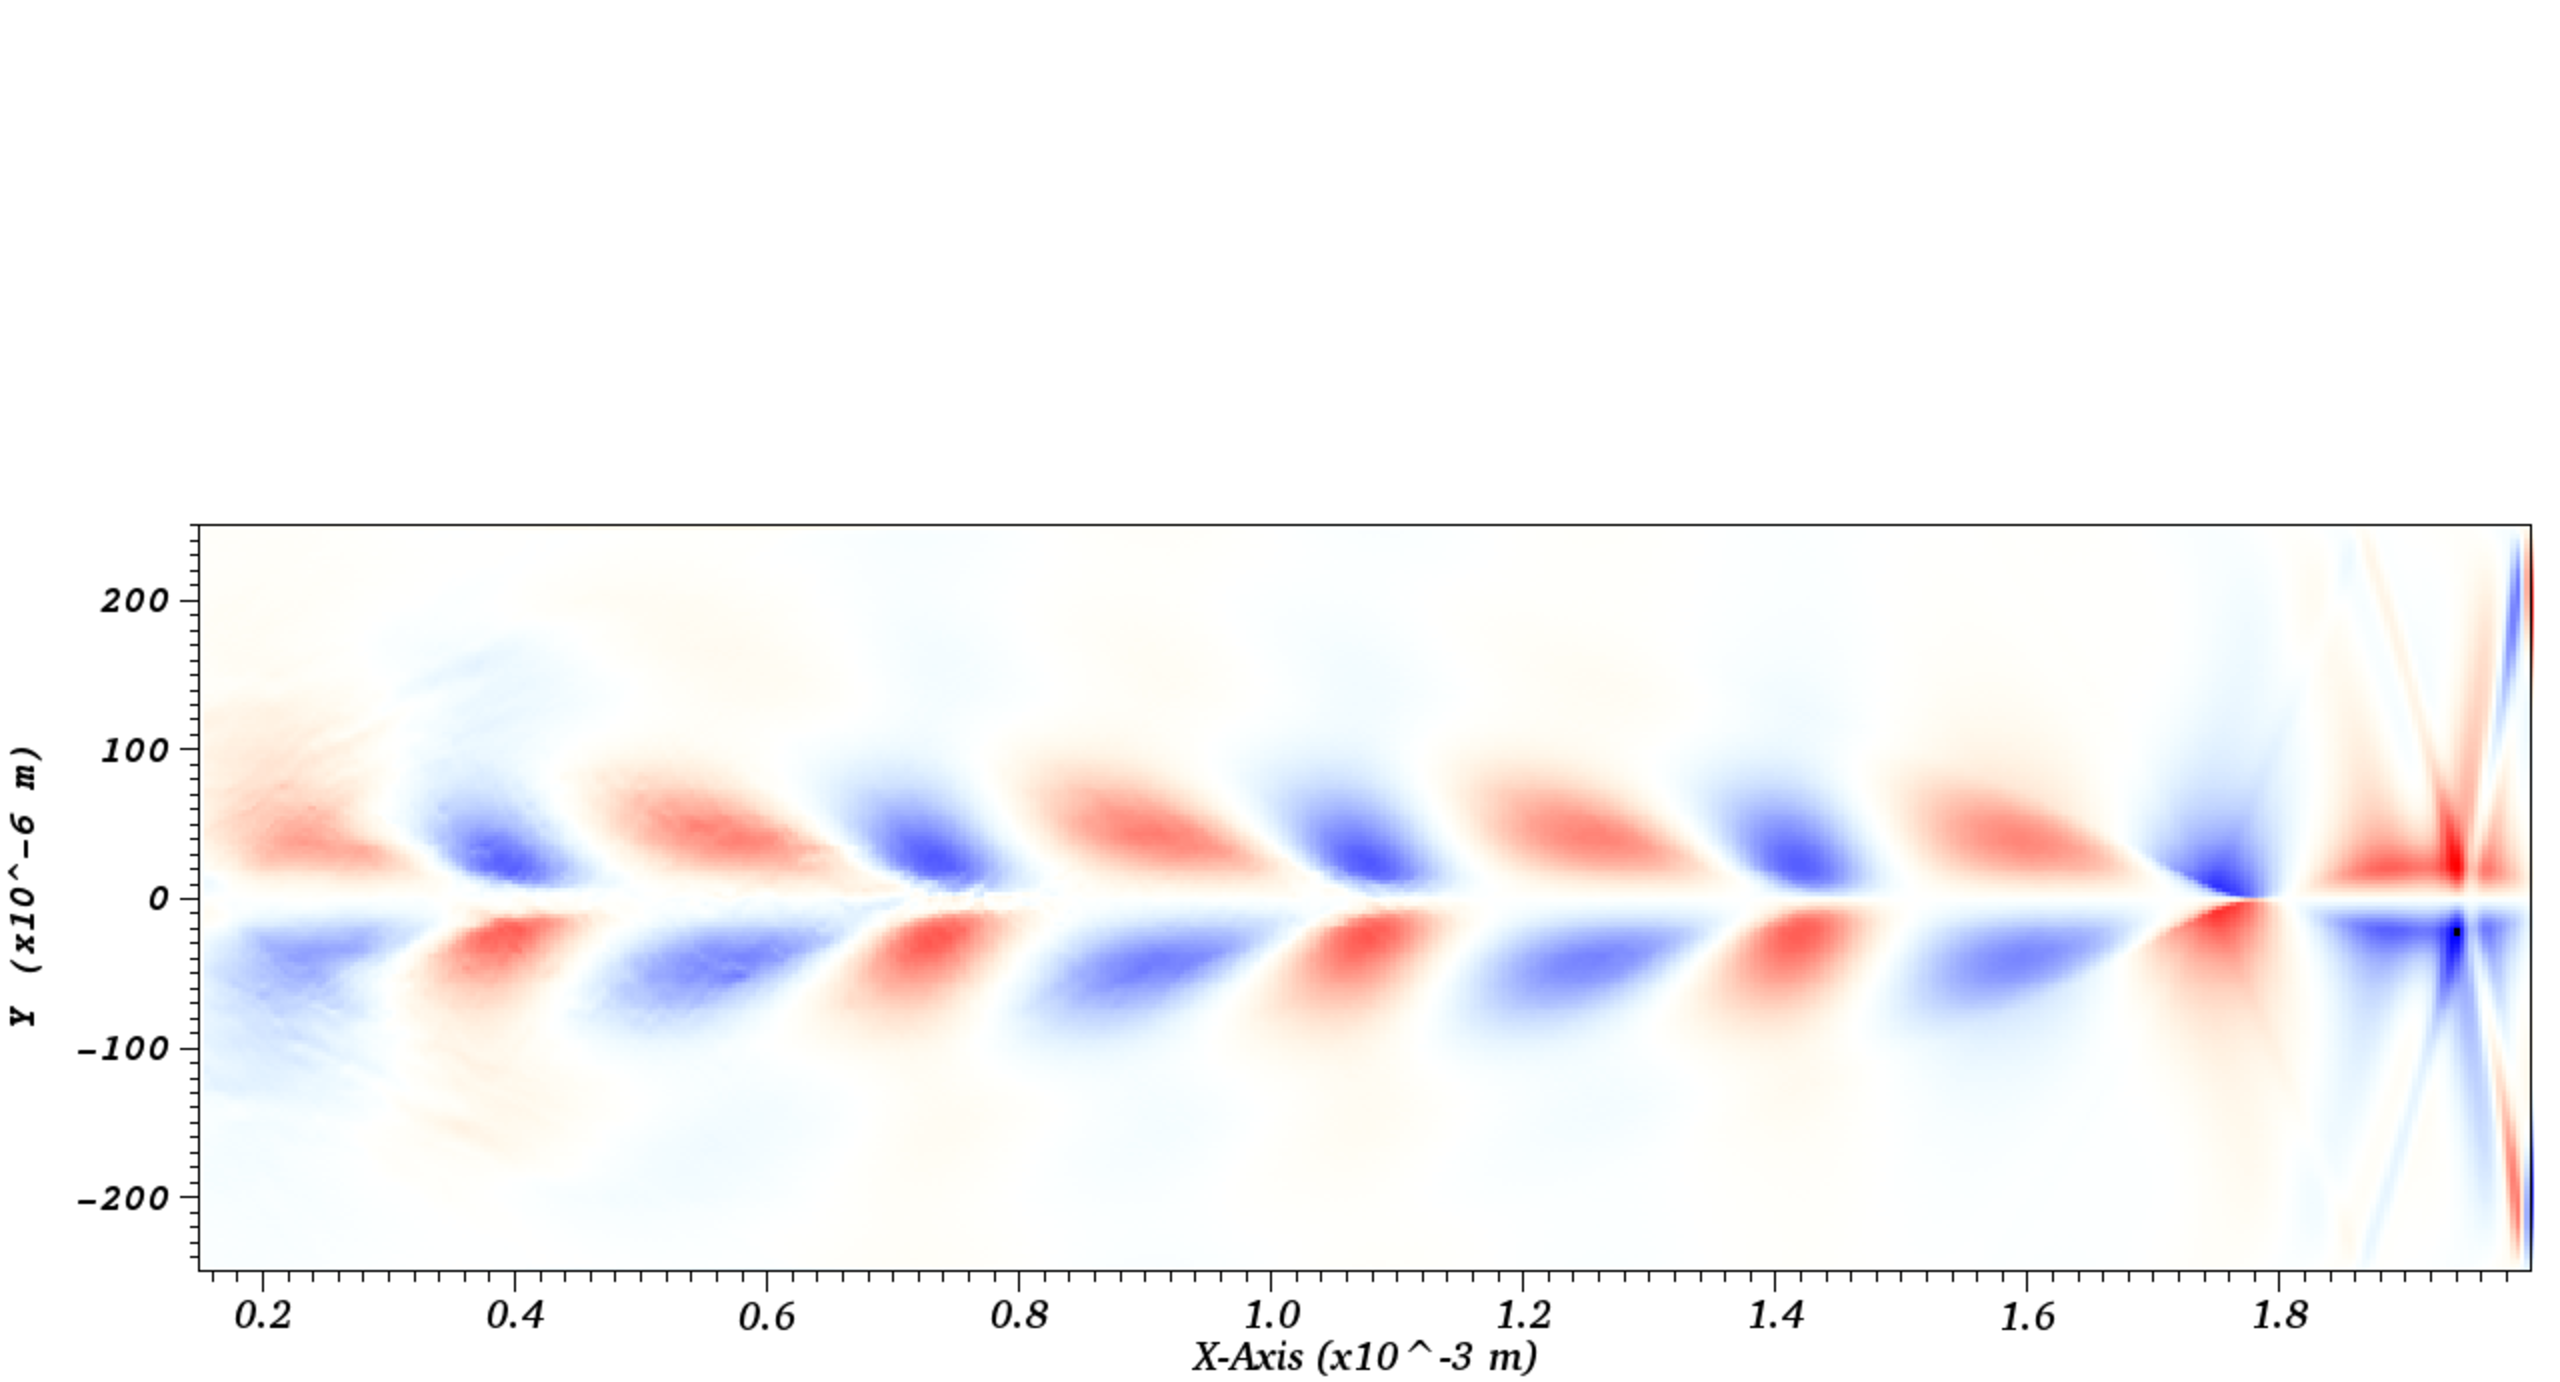
\includegraphics[width=\textwidth]{Ey_nonlinear.png}
\caption{Should these three plots be in results or here? OR PUT SIMUALTIONS CHAPTER BEFORE THEORY CHAPTER. Then theory can be used to also verify that simulations work. Probably not, better explain everything to motivate what simulations to be done }
\end{figure}
\begin{equation}
-\left(\frac{\mathrm{d}E}{\mathrm{d}z}\right)_{\text{coll-wave-break}}=F_e=eE_{wave-break}=m_e c\omega_{p}\left(\frac{n_b}{n_e}\right)
\end{equation}

What is the wave-breaking electric field?

\section{Notes.}
Meeting Guoxing:
\begin{itemize}
\item We will change $\sigma_{x,y}$, in simulation from $\sigma_{x,y}=0.3 \mu m ~\to~5-10 \mu m$ because the $0.3\mu m$ EuPRAXIA beam parameter gives to high beam density $n_b$, which means that we can't have $n_b\sim n_p$ because the plasma density would have to be too high. We should aim for $n_p\sim 10^{17}-10^{18}\sim n_b$ (standard L/PWFA) parameters. 
EuPRAXIA wants $\sigma_{x,y}$ small because small bunches gives more coherent radiation in undulators. One could expand the beam by letting it propagate freely (expand due to space charge) a distance before reaching the beam dump. 
\item $\text{Run simulations with uniform plasma density for }\left\{\begin{aligned}
&n_p\sim 0.1 n_b \quad &&\text{Non-linear}\\
&n_p\sim  n_b\quad &&\text{Quasi-linear}\\
&n_p\sim 10 n_b\quad &&\text{Linear}
\end{aligned}\right.$ \\
\item Use $\Delta E/E=0.01$ and bunch charge $30~$pC ($5~$fs).\\
\item Estimate necessary simulation propagation length by saturation length using wave-breaking electric field gradient 
$$L_{\text{sat}}\approx \frac{T_0}{eE_{wb}}=\frac{T_0}{e}\frac{e}{m_e c\omega_p}=\frac{T_0}{m_e c}\sqrt{\frac{m_e e\epsilon_0}{e^2n_b}} $$ 
\item Project outline:
\begin{itemize}
\item Uniform plasma with varying $n_b\sim n_p$
\item Vary plasma density profile
\item Test laser to dump head of beam
\item Run simulations for real FlashForward parameters and not the idealized EuPRAXIA parameters.
\end{itemize}
\item  100pC $$n_b=\frac{N_p}{(2\pi)^{3/2} \sigma_y^2\sigma_x}=\frac{6.25\times 10^{8}}{(2\pi)^{3/2} (5\times 10^{-6})^3}\approx 3.2\times 10^{23}~ \text{m}^{-3} $$
$$\Rightarrow ~~eE_{\text{wb}}=\left\{\begin{aligned}
&17 ~\text{GeV/m }&& n_p=0.1 n_b \\
&54 ~\text{GeV/m} && n_p=n_b\\
&172 ~\text{GeV/m} &&n_p=10 n_b
\end{aligned}\right.\quad\Rightarrow ~~L_{sat}(1 ~\text{GeV})=\left\{\begin{aligned}
&5.8 ~\text{cm}&& n_p=0.1 n_b \\
&1.9 ~\text{cm} && n_p=n_b\\
&0.6 ~\text{cm} &&n_p=10 n_b
\end{aligned}\right.$$
$$1 ~\text{GeV beam} ~~\Rightarrow ~~ L_{sat}\sim 2 ~\text{cm}=2*10^4 \mu \text{m} $$
\item  30pC $$n_b=\frac{N_p}{(2\pi)^{3/2} \sigma_y^2\sigma_x}=\frac{1.87\times 10^{8}}{(2\pi)^{3/2} (5\times 10^{-6})^3}\approx 9.5\times 10^{22}~ \text{m}^{-3} $$
$$\Rightarrow ~~eE_{\text{wb}}=\left\{\begin{aligned}
&9.4 ~\text{GeV/m }&& n_p=0.1 n_b \\
&30 ~\text{GeV/m} && n_p=n_b\\
&94 ~\text{GeV/m} &&n_p=10 n_b
\end{aligned}\right.\quad\Rightarrow ~~L_{sat}(1 ~\text{GeV})=\left\{\begin{aligned}
&10.7 ~\text{cm}&& n_p=0.1 n_b \\
&3.4 ~\text{cm} && n_p=n_b\\
&1.1 ~\text{cm} &&n_p=10 n_b
\end{aligned}\right.$$
$$1 ~\text{GeV beam} ~~\Rightarrow ~~ L_{sat}\sim 3.4 ~\text{cm}=3.4*10^4 \mu \text{m} $$



\clearpage
\begin{verbatim}
ExportDBAtts = ExportDBAttributes()
ExportDBAtts.allTimes = 0
ExportDBAtts.dirname = "/Users/oscarjakobsson/Documents/epoch-4.14.4/epoch2d"
ExportDBAtts.filename = "test"
ExportDBAtts.timeStateFormat = "_%04d"
ExportDBAtts.db_type = "Xmdv"
ExportDBAtts.db_type_fullname = "Xmdv_1.0"
ExportDBAtts.variables = ("Particles/Ek/edriver", "Particles/Weight/edriver")
ExportDBAtts.writeUsingGroups = 0
ExportDBAtts.groupSize = 48
ExportDBAtts.opts.types = (0)
ExportDBAtts.opts.help = ""
ExportDatabase(ExportDBAtts)
ExportDBAtts = ExportDBAttributes()
ExportDBAtts.allTimes = 0
ExportDBAtts.dirname = "/Users/oscarjakobsson/Documents/epoch-4.14.4/epoch2d"
ExportDBAtts.filename = "test"
ExportDBAtts.timeStateFormat = "_%04d"
ExportDBAtts.db_type = "Xmdv"
ExportDBAtts.db_type_fullname = "Xmdv_1.0"
ExportDBAtts.variables = ("Particles/Ek/edriver", "Particles/Weight/edriver")
ExportDBAtts.writeUsingGroups = 0
ExportDBAtts.groupSize = 48
ExportDBAtts.opts.types = (0)
ExportDBAtts.opts.help = ""
ExportDatabase(ExportDBAtts)

\end{verbatim}

\begin{itemize}
\item Issue: restart not possible with laser. 
\item EPOCH allows for a user to manually override particle-parameter distributions defined in the input deck, in which all functions must be defined analytically. By overriding this so-called autoloader, which takes the analytical distributions in the input deck and distributes the macro particles accordingly, this manual approach allows for the initialisation of a bunch with non-analytical density and momentum distributions. 
\item Furthermore, even if the density distribution were to be easily described analytically, this method offers the advantage that it also overrides the maxwellian velocity distribution that epoch assigns to each bunch of particles in the input deck. This is fine for an initial bunch in thermal equilibrium, but as soon as plasma interaction occurs the velocity distribution of the electrons in the bunch is noticeably non-maxwellian
\item VisIt - export data from .sdf file, convert to -csv, read with ic module when compiling epoch.
\item (show below, it is possible to have a laser appear before the bunch at some time t, but the parameters of this laser could not be changed so testing several differnt laser intensities, distances etc. would take far too long if the bunch was forced to propagate 20cm each time before the laser was ramped up )
\end{itemize}

\subsection{Input deck}
Once EPOCH has been downloaded and compiled the so-called input deck is essentially EPOCH's user interface. This is a file in which users specify the details of a simulations and it is this file that gets read by EPOCH and passed onto the core PIC algorithm. The input deck consists of blocks which define parameters for different features of the simulation. \\
\textbf{Explain control block first}, and what the restart does.
\begin{verbatim}
begin:control
  dlb_threshold = 0.5
  restart_snapshot=restartXXXX.sdf
  t_end = end_time
  nx = nint(length / cell_length)
  ny = nint((half_width * 2) / cell_width)
  npart = part_per_cell * nx * ny
  stdout_frequency = 50
  use_random_seed = T
end:control
\end{verbatim}
This specifies the grid that the simulations is to run on. We then populate this grid with plasma particles.
\textbf{Species block}, with explanation about analytical density distributions for plasma, and specify ppc.\\
The control and species blocks together define the resolution of the simulation. When setting up the resolution of the grid one has to make sure that the grid is sufficiently fine such that the smallest features of our physical system are resolved. This is to ensure that the simulation accurately models the physical system it is meant to represent, to the extent that missing small scale phenomena might alter the large scale outcome of the simulation. A finer grid however requires more macroparticles to fully populate the grid, which inevitably extents the computational time. In addition the time step $\Delta t$ aneeds to be suitably decreased as well. This is because of the so-called Courant-Friedrichs-Lewy (CFL) condition.  Any simulation introduces uncertainties in the final outcome due to the finite resolution. We need to make sure that the uncertainties introduces during each iteration do not build up and grow unbounded. \\
\\
\textbf{edriver} with analytical distribution, and laser, followed by boundaries
\begin{center}
\begin{verbatim}
begin:boundaries
  bc_x_min = simple_laser
  bc_x_max = simple_outflow
  bc_y_min = simple_outflow
  bc_y_max = simple_outflow
end:boundaries
\end{verbatim}
\end{center}
\textbf{output block} and the sdf file visualisation with VisIT

%Parameters and initial conditions are defined using an \textit{input.deck} file.

%$$n_b = \frac{1}{{\sigma_x\sigma_y^2 (2\pi)^{3/2 }  }}e^{{{ - \left( {x - x_0 } \right)^2 } \mathord{\left/ {\vphantom {{ - \left( {x - x_0 } \right)^2 } {2\sigma_x ^2 }}} \right. \kern-\nulldelimiterspace} {2\sigma_x^2 }}}e^{{{ - \left( {y - y_0} \right)^2 } \mathord{\left/ {\vphantom {{ - \left( {y- y_0 } \right)^2 } {2\sigma_y ^2 }}} \right. \kern-\nulldelimiterspace} {2\sigma_y ^2 }}}e^{{{ - \left( {y - y_0 } \right)^2 } \mathord{\left/ {\vphantom {{ - \left( {y - y_0 } \right)^2 } {2\sigma ^2 }}} \right. \kern-\nulldelimiterspace} {2\sigma_y ^2 }}}$$




\indent Given that a plasma is no more than electrons and ions interacting electromagnetically, the response of such a plasma to the propagation of an electron bunch or laser pulse could in theory be simulated by solving Maxwell's equations for a set of initial conditions. This would involve solving Maxwell's equations at time an initial time $t_0$ and calculating the combined electromagnetic fields acting on each particle in the plasma. Then, by considering each particles velocity, one could calculate the new positions and velocities of all particles for a small time increase $t_0+\Delta t$. Repeating these computation would  lead us to find the approximate plasma response at any arbitrary time $t>t_0$. However, this approach is computationally intractable. Since if we attempt this approach in most plasma simulations. For instance, if we consider that the plasma in a typical plasma wakefield accelerator [Hanahoe] is on the order of centimetres in extent, with a number density $~10^{20} m^{-3}$, we find that we have on the order of $10^{14}$ electrons in the plasma. All these electrons would have to be included in the simulation and stored with their associated 6-dimensional position and velocity data $(x,y,z,v_x,v_y,v_z)$. Each number would be stored as a 32-bit double precision floating point number, yielding the total data size required for the whole plasma simulation on the order of a petabyte ($10^{15}$ bytes).\\





\section{Particle-in-Cell Codes}
\label{sec:Particle-in-Cell Codes}
Starting from EM fields $\vec{E}_{(n)},\vec{B}_{(n)}$ and charge current $\vec{J}_{(n)}$ present at iteration $n$ [at a specific position, middle of Yee grid?] we obtained the fields at the next time step $n+1$ by computing the resulting fields and currents at an intermediate half-way step $n+1/2$. We do this by first computing the change in the electric field, using Ampere's law, $\Delta \vec{E}_{(n)}$ which we add to our current field such that
\begin{equation}
\vec{E}_{(n+1/2)}=\vec{E}_{(n)}+\frac{\Delta t}{2}\left(c^2\mathbf{\nabla}\times \vec{B}_{(n)}-\frac{\vec{J}_{(n)}}{\epsilon_0}\right)
\end{equation}
from this the magnetic field is given by
\begin{equation}
\vec{B}_{(n+1/2)}=\vec{B}_{(n)}-\frac{\Delta t}{2}\left(c^2\mathbf{\nabla}\times \vec{E}_{(n+1/2)}\right)
\end{equation}
(at which point the particle pusher, detailed below, updates the current to $\vec{J}_{(n+1)}$)\\
at which point we need to update the current to $\vec{J}_{(n+1)}$ in order to proceed finding the fields at time step $n+1$. This is done using the particle pusher. We update the position of each particle 
\begin{equation}
\vec{x}_{(n+1/2)}=\vec{x}_{(n)}+\frac{\Delta t}{2}\vec{v}_{(n)}
\end{equation}
from which we also obtain the intermediate velocity $\vec{v}_{(n)}$ [correct?]. Using the Lorentz force law we then compute the force $\vec{F}_{(n)}=\Delta p/\Delta t$ which gives the momentum at $n+1$ as
\begin{equation}
\vec{p}_{(n+1)}=\vec{p}_{(n)}+q\Delta t\left[\vec{E}_{(n+1/2)}\left(\vec{x}_{(n+1/2)}\right)+\vec{x}_{(n+1/2)}\times\vec{B}_{(n+1/2)}\left(\vec{x}_{(n+1/2)}\right) \right]
\end{equation}
where, the electric fields are extrapolated (?) to the intermediate point $n+1/2$. Then, using $\vec{p}=\gamma m \vec{v}$, we can find the velocity at $n+1$, from which we then have the current $\vec{J}_{(n+1)}$. We then reverse the order of computing such that the magnetic field is calculated prior to the electric field,
\begin{align}
&\vec{B}_{(n+1)}=\vec{B}_{(n+1/2)}-\frac{\Delta t}{2}\left(c^2\mathbf{\nabla}\times \vec{E}_{(n+1/2)}\right)\\
&\vec{E}_{(n+1)}=\vec{E}_{(n+1/2)}+\frac{\Delta t}{2}\left(c^2\mathbf{\nabla}\times \vec{B}_{(n+1)}-\frac{\vec{J}_{(n+1)}}{\epsilon_0}\right)
\end{align}
Using these fields when then calculate the new particles positions $\vec{x}_{(n)}$, we "push" the particles, thus completing the iteration step.








\clearpage 
Particles are not on yee grid but fields are on yee grid. So rho and J need to be put on yee grid to find fields, and to find new particle positions the fields need to be calculated off-yee grid. However, since the electric field is sourced in part by magnetic flux variations, the fields are sovled at intermediate steps.\\
Since the fields are determined by the position and velocity of the particles, which in turn are determined by the fields, these can not be calculated simulataneously. In its simpelest form, PIC codes decouple these calculations by dividing each iterations step into four seperate parts.  
EM fields are fixed on grid, particles move freely
\label{sec:Particle-in-Cell Codes}
Starting from EM fields $\vec{E}_{(n)},\vec{B}_{(n)}$ and charge current $\vec{J}_{(n)}$ present at iteration $n$ [at a specific position, middle of Yee grid?] we obtained the fields at the next time step $n+1$ by computing the resulting fields and currents at an intermediate half-way step $n+1/2$. We do this by first computing the change in the electric field, using Ampere's law, $\Delta \vec{E}_{(n)}$ which we add to our current field such that
\begin{equation}
\vec{E}_{(n+1/2)}=\vec{E}_{(n)}+\frac{\Delta t}{2}\left(c^2\mathbf{\nabla}\times \vec{B}_{(n)}-\frac{\vec{J}_{(n)}}{\epsilon_0}\right)
\end{equation}
from this the magnetic field is given by
\begin{equation}
\vec{B}_{(n+1/2)}=\vec{B}_{(n)}-\frac{\Delta t}{2}\left(c^2\mathbf{\nabla}\times \vec{E}_{(n+1/2)}\right)
\end{equation}
(at which point the particle pusher, detailed below, updates the current to $\vec{J}_{(n+1)}$)\\
at which point we need to update the current to $\vec{J}_{(n+1)}$ in order to proceed finding the fields at time step $n+1$. This is done using the particle pusher. We update the position of each particle 
\begin{equation}
\vec{x}_{(n+1/2)}=\vec{x}_{(n)}+\frac{\Delta t}{2}\vec{v}_{(n)}
\end{equation}
from which we also obtain the intermediate velocity $\vec{v}_{(n)}$ [correct?]. Using the Lorentz force law we then compute the force $\vec{F}_{(n)}=\Delta p/\Delta t$ which gives the momentum at $n+1$ as
\begin{equation}
\vec{p}_{(n+1)}=\vec{p}_{(n)}+q\Delta t\left[\vec{E}_{(n+1/2)}\left(\vec{x}_{(n+1/2)}\right)+\vec{x}_{(n+1/2)}\times\vec{B}_{(n+1/2)}\left(\vec{x}_{(n+1/2)}\right) \right]
\end{equation}
where, the electric fields are extrapolated (?) to the intermediate point $n+1/2$. Then, using $\vec{p}=\gamma m \vec{v}$, we can find the velocity at $n+1$, from which we then have the current $\vec{J}_{(n+1)}$. We then reverse the order of computing such that the magnetic field is calculated prior to the electric field,
\begin{align}
&\vec{B}_{(n+1)}=\vec{B}_{(n+1/2)}-\frac{\Delta t}{2}\left(c^2\mathbf{\nabla}\times \vec{E}_{(n+1/2)}\right)\\
&\vec{E}_{(n+1)}=\vec{E}_{(n+1/2)}+\frac{\Delta t}{2}\left(c^2\mathbf{\nabla}\times \vec{B}_{(n+1)}-\frac{\vec{J}_{(n+1)}}{\epsilon_0}\right)
\end{align}
Using these fields when then calculate the new particles positions $\vec{x}_{(n)}$, we "push" the particles, thus completing the iteration step.






The hybrid scheme approach that the endeavour to investigate in this project relies on us being able to simulate a laser pulse propagating in front of a pre-saturated bunch. Previous investigations by our colleagues have shown that this is not a trivial task using the simulation software that have been tried. The issue with epoch in this regard is that everything that is to be included in the simulation need to be specified in the input deck and introduced at the beging of a simulation. Hence, simulations of the active beam dump are entirely possible in EPOCH, since a laser can be initialised in front of a bunch at $t=0$ and driven together. Introducing a laser at a later stage $t>0$ appeared however not to be possible. The majority of the work so far in this project has been concerned with solving this issue. The approach taken was to simulate the passive part first and then export the data of the saturated bunch into a new simulation which includes a laser driver. The structure of the SDF data files output by EPOCH are however not suitable for accessing and retrieving particular sets of data. A workaround was found by using VisIt to read the files and subsequently export only the data related to the electron beam. This data was subsequently read by EPOCH during the compilation stage in a specific file included in EPOCH. This file, usually left empty, allows users to over-ride section of the input file by assigning custom values to each of the macroparticles that are intialised in at the start of a simulation. Through this approach we are now able to define a simulation where a laser pulse is driven ahead of a standard bi-gaussian electron beam. By then over-riding the parameters for the electron beam we can then use the data from a pre-saturated bunch to reposition each macroparticle in the bi-gaussian to its corresponding position relative to the rest of the bunch. By also over-riding momentum parameters we can completely mould the bunch into the one we had exported after a passive beam dump. \\
\\
Real accelerators operate at a range of beam parameters tailored to specific reserach purposes. In order to avoid having to set up week-long simulations for each minor change of parameters it is crucial to understand the theory underlying these plasma wakefield phenomena and to see to what extent the theoretical predictions match the simulations

For any pracitactal implementation of the hybrid scheme to an existing experiment it 


%\subsection{Notes Bonatto}
%Rate of change due to the longitudinal electric field acting on an electron beam, i.e position beam in the decelerating region of the wakefield.\\
%"the beam only experiences its self-excited wakefield."\\
%In the passive beam dump, are we essentially slowing down a "drive bunch" without having a witness bunch behind to get accelerated?\\
%It is probaly better to u se gamma as in Bonatto's paper, to make it easier to explain total beam energy integral. Basically integrate over all particles.\\
%$U=\gamma m_ec^2$
%\begin{equation}
%-\frac{\mathrm{d}U}{\mathrm{d}s}=(F_e)_z=eE_z
%\end{equation}
%where $s$ is the distance travelled in the plasma and $U$ is the energy of a particle in the beam at position $\xi$. 
%for ultra relativistic beams, $\beta\sim 1$, the longitudinal electric field is a function of the position along the bunch $\xi=z-ct$ and not $z$ explicitly. 
%\begin{equation}
%U(s,\xi)=U_0-esE_z(\xi)
%\end{equation}
%The total energy of the beam after travelling a distance $s$ is then found by integrating across all the particles in the beam, which is integrating across $\xi$ since analysis is in 1-D.
%\begin{equation}
%\mathcal{U}(s)=U_0\int_{-\infty}
%\end{equation}

%We will proceed by calculating the gamma factor of a given particle in the beam who's energy we wish to compute.
%\begin{equation}
%\gamma(s,\xi)=\gamma_0-esE_z(\xi)
%\end{equation}

%Based on the work of Lu et. al \citep{Lu2006}, wherein it was shown that the predictions from the linear models perform well even in the non-linear regime, it is of interest to compute the energy loss in the linear regime. 

%\section{Non-linear Regime} 
%Lower density, larger plasma response, not possible to describe perturbatively. Hamiltonian approach taken by Lu. et al []\\
%Self-injection?